\documentclass[../CSC_5RO06_TA.tex]{subfiles}
\usepackage{makecell}

\begin{document}
\section*{Question 1}

\subsection{Caractéristiques de l'ordinateur utilisé}

La configuration de l'environnement se trouve dans le tableau suivant.

\begin{table}[h]
    \centering
    \begin{tabular}{c|c}
        \hline
        Processeur & \makecell{Intel(R) Core(TM) i5-1135G7\\ de 11ème génération} \\ \hline
        Nombre de cœurs & 4\\ \hline
        Nombre de processeurs & 8\\ \hline
        Fréquence & 2.40 GHz  \\ \hline
        Mémorie & 8 Go de RAM  \\ \hline
        Système d'exploitation & Windows 11  \\ \hline
        Compilateur & GNU GCC Compiler 13.2.0 \\
        \hline   
    \end{tabular}
    % \caption{Caption}
    \label{tab:my_label}
\end{table}

\subsection{Optimisation du compilateur gcc}

Dans un premier temps, nous avons voulu examiner comment les optimisations conçues par le compilateur gcc pourraient améliorer les performances des algorithmes de multiplication matricielle vus précédemment.

Premièrement, le système a été exécuté sans optimisation (O0), de sorte que les algorithmes seraient exécutés comme décrit dans le code utilisé. Ci-dessous, vous pouvez consulter les résultats du temps d'exécution pour chacun des algorithmes avec différentes tailles de matrice.

\begin{figure}[H]
    \centering
    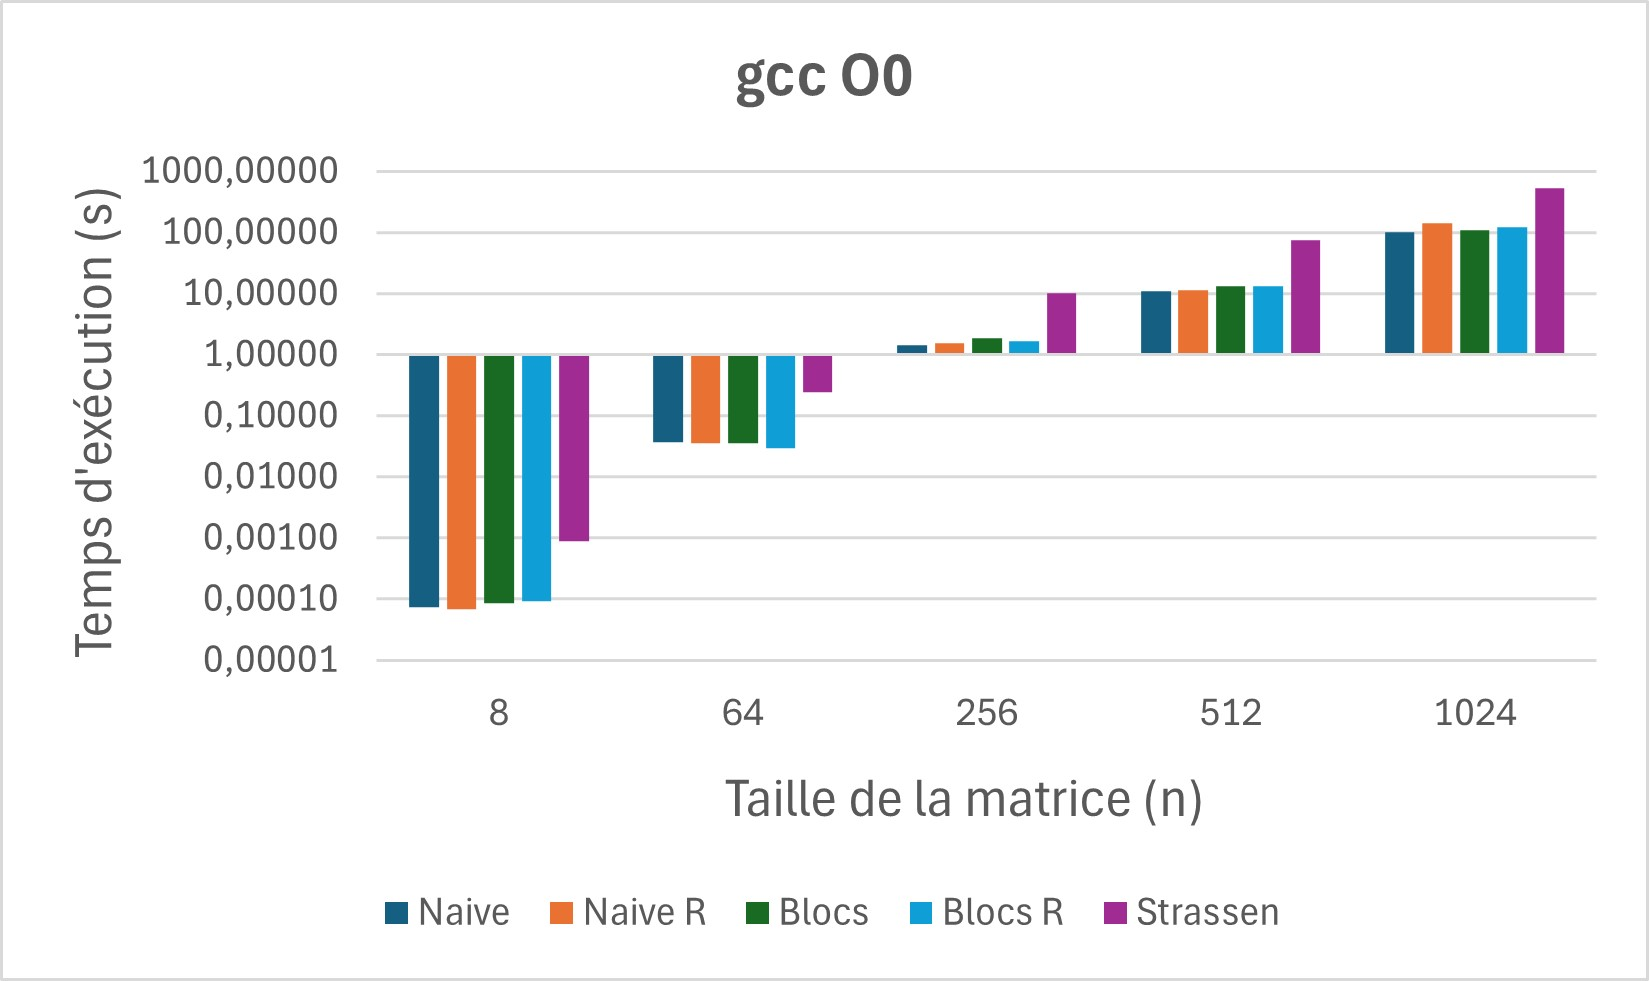
\includegraphics[width=1\columnwidth]{Images/Temps_gcc0.jpg}
    \caption{Temps d'exécution de l'algorithme avec optimisation gcc O0.}
    \label{fig:1}
\end{figure}


Une fois connaissant les résultats du système sans optimisation, nous avons procédé à tester chacune des 3 options de parallélisation, et à mesurer leur Speed Up par rapport au programme sans optimisation.

\subsubsection{gcc O1}

Effectue des optimisations simples qui n'augmentent pas significativement le temps de compilation. Cela inclut des optimisations telles que la suppression du code inutilisé, la simplification des expressions et certaines optimisations de boucles. L'objectif est d'améliorer les performances sans compliquer le processus de compilation.

Les résultats avec cette configuration peuvent être vus ci-dessous.

\begin{figure}[H]
    \centering
    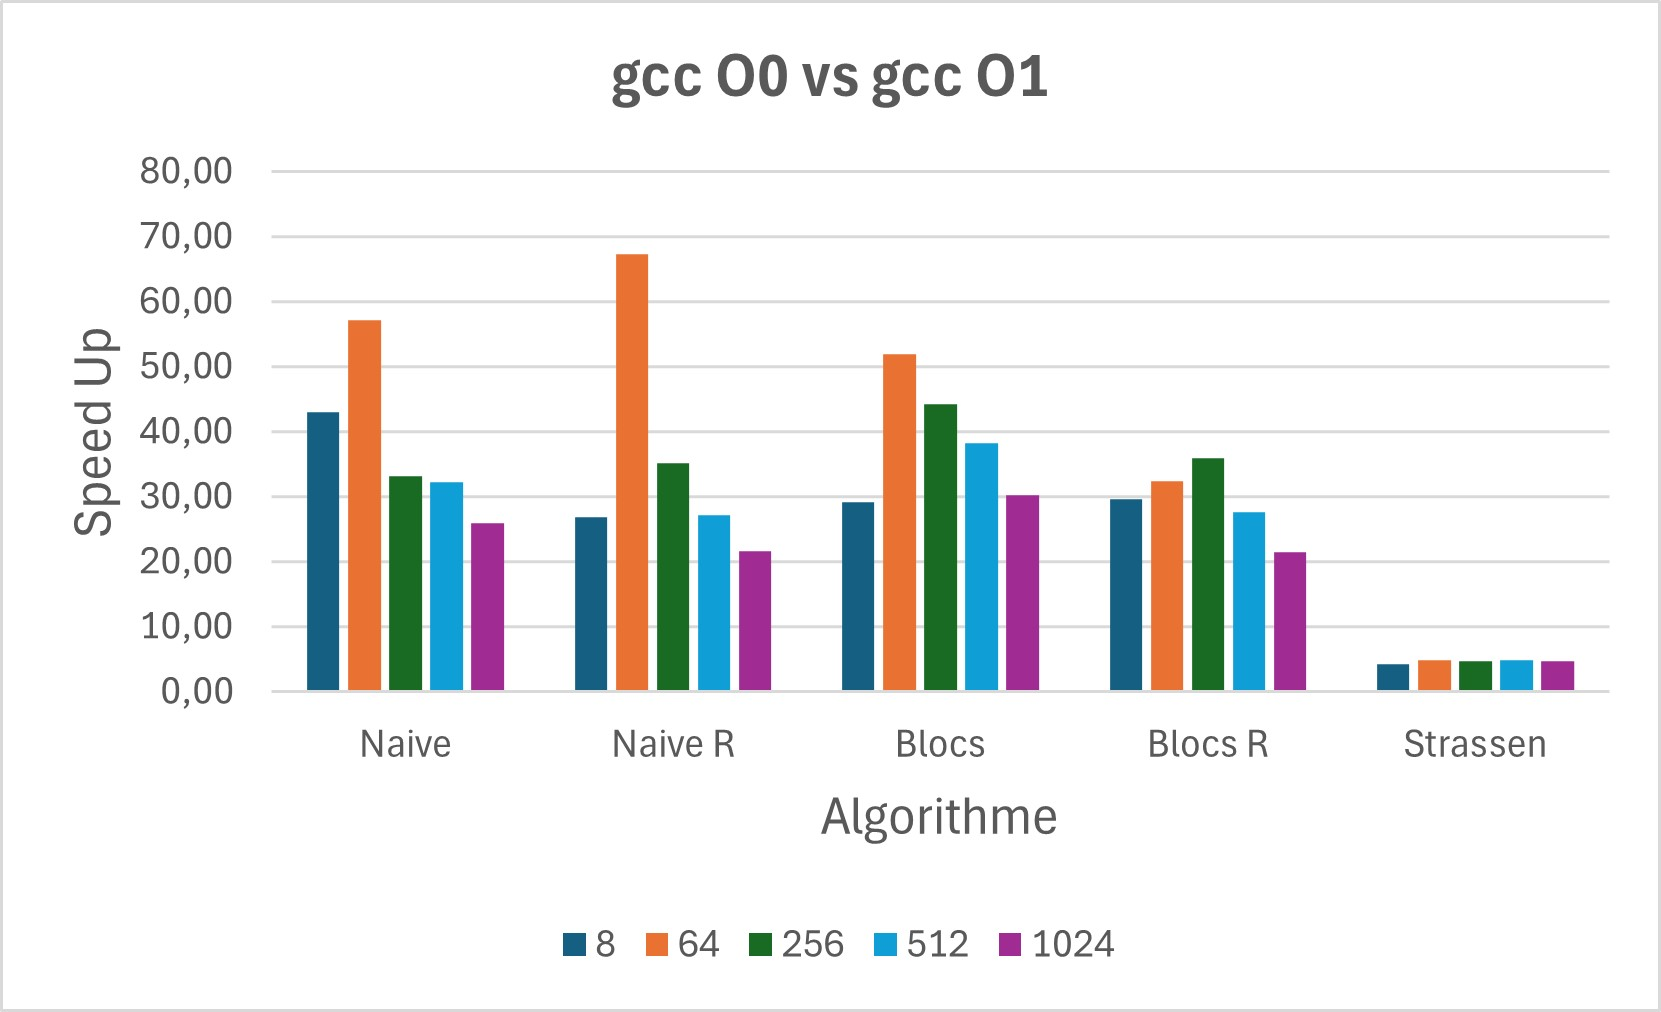
\includegraphics[width=1\columnwidth]{Images/SpeedUp1_gcc0vsgcc1.jpg}
    \caption{Speed Up de l'optimisation de gcc O1 par rapport à gcc O0.}
    \label{fig:2}
\end{figure}

L'optimisation O1 améliore considérablement les performances dans presque tous les algorithmes, en particulier pour les matrices plus petites (8x8), où l'algorithme Naïve présente une forte augmentation. En effet, O1 applique de légères optimisations telles que la suppression du code mort et une réutilisation améliorée des registres, mais sans réorganisation agressive du code, tout en maintenant une bonne cohérence de l'accès à la mémoire. Dans des algorithmes plus complexes comme Strassen, l’accélération est plus faible, ce qui suggère que la nature récursive de l’algorithme limite les avantages de O1.

\subsubsection{gcc O2}

Comprend toutes les optimisations O1, ainsi que des optimisations plus avancées. Celles-ci peuvent inclure l’extension des fonctions en ligne, l’optimisation de boucles plus complexes et l’amélioration de l’utilisation de la mémoire. Il recherche un équilibre entre performances et temps de compilation, offrant un code plus efficace sans trop compromettre le temps de compilation.

La figure ci-dessous montre le Speed Up par rapport à la configuration sans optimisation.

\begin{figure}[H]
    \centering
    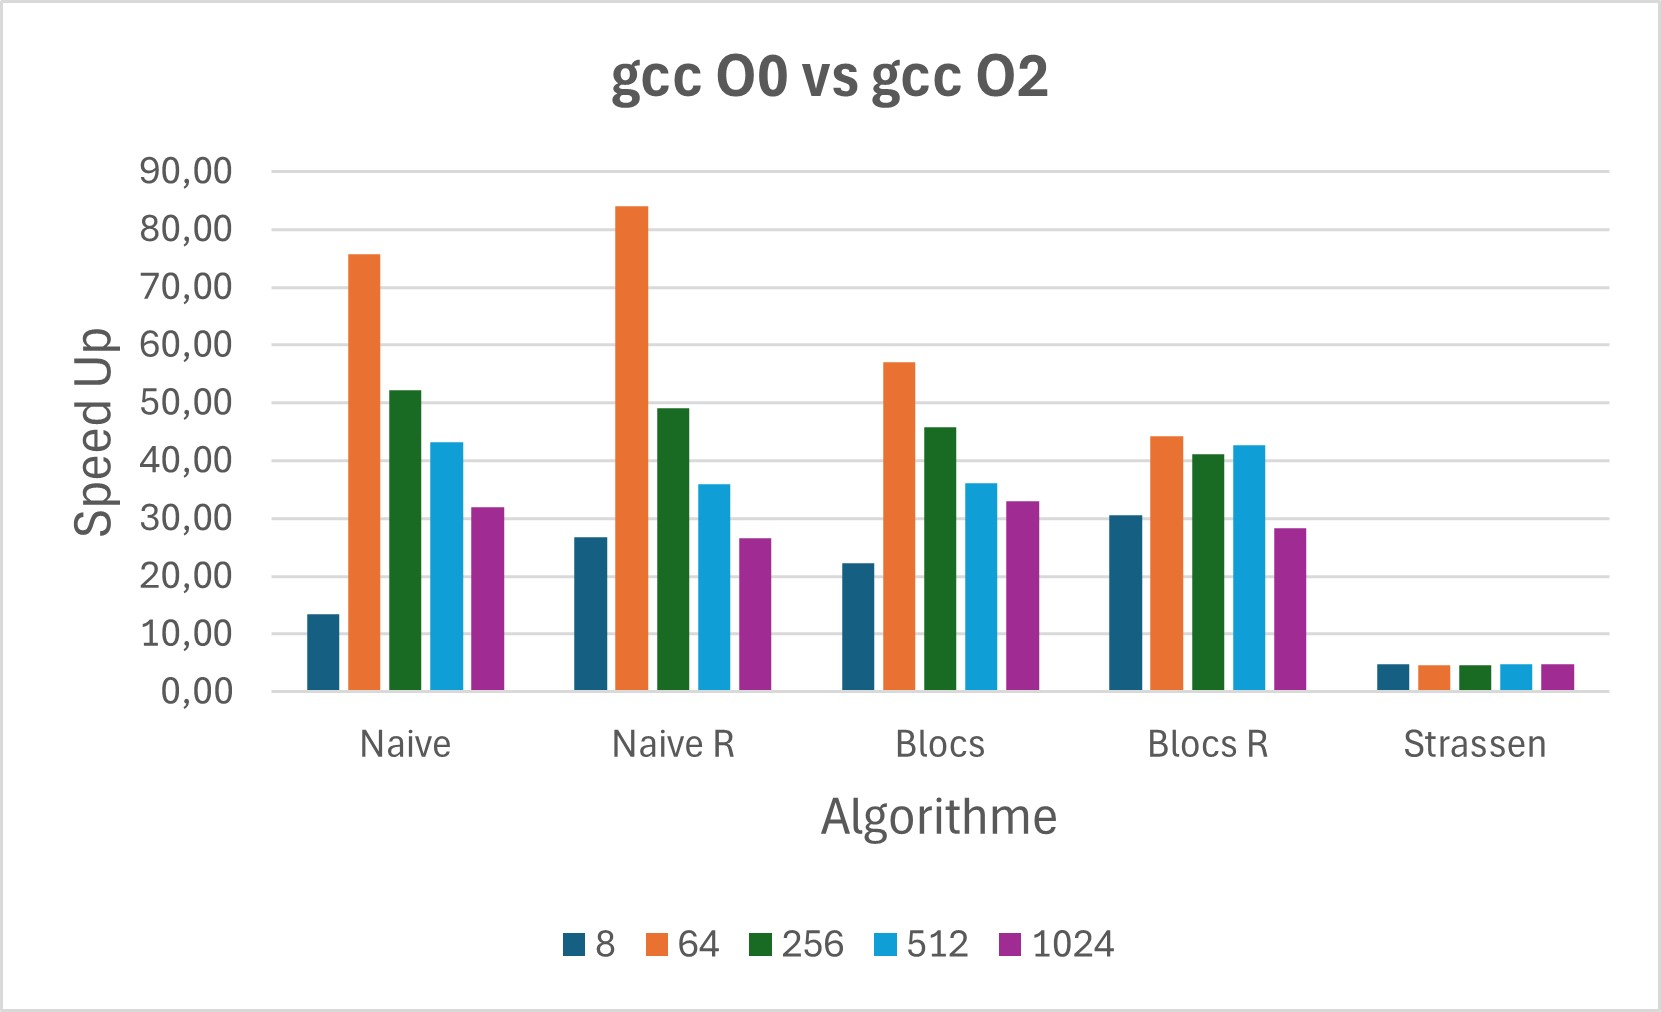
\includegraphics[width=1\columnwidth]{Images/SpeedUp1_gcc0vsgcc2.jpg}
    \caption{Speed Up de l'optimisation de gcc O2 par rapport à gcc O0.}
    \label{fig:3}
\end{figure}

L'optimisation O2 montre des améliorations encore plus prononcées, en particulier sur les matrices de taille moyenne comme 64x64 et 256x256, où brillent les algorithmes de réorganisation et de bloc. Cela est dû à des optimisations O2 plus agressives, notamment la vectorisation, la réorganisation du code et la réduction de la pression du cache. Les techniques de prélecture et de réorganisation des boucles font un meilleur usage de l'accès mémoire, même si l'amélioration est plus modeste pour Strassen, puisque ses sous-problèmes ne bénéficient pas autant de ces optimisations.

\subsubsection{gcc O3}

Inclut toutes les optimisations O2 et se concentre sur l’amélioration supplémentaire des performances au détriment du temps de compilation. Cela peut inclure des techniques telles que la vectorisation et l'unification des boucles.

Ci-dessous les résultats.

\begin{figure}[H]
    \centering
    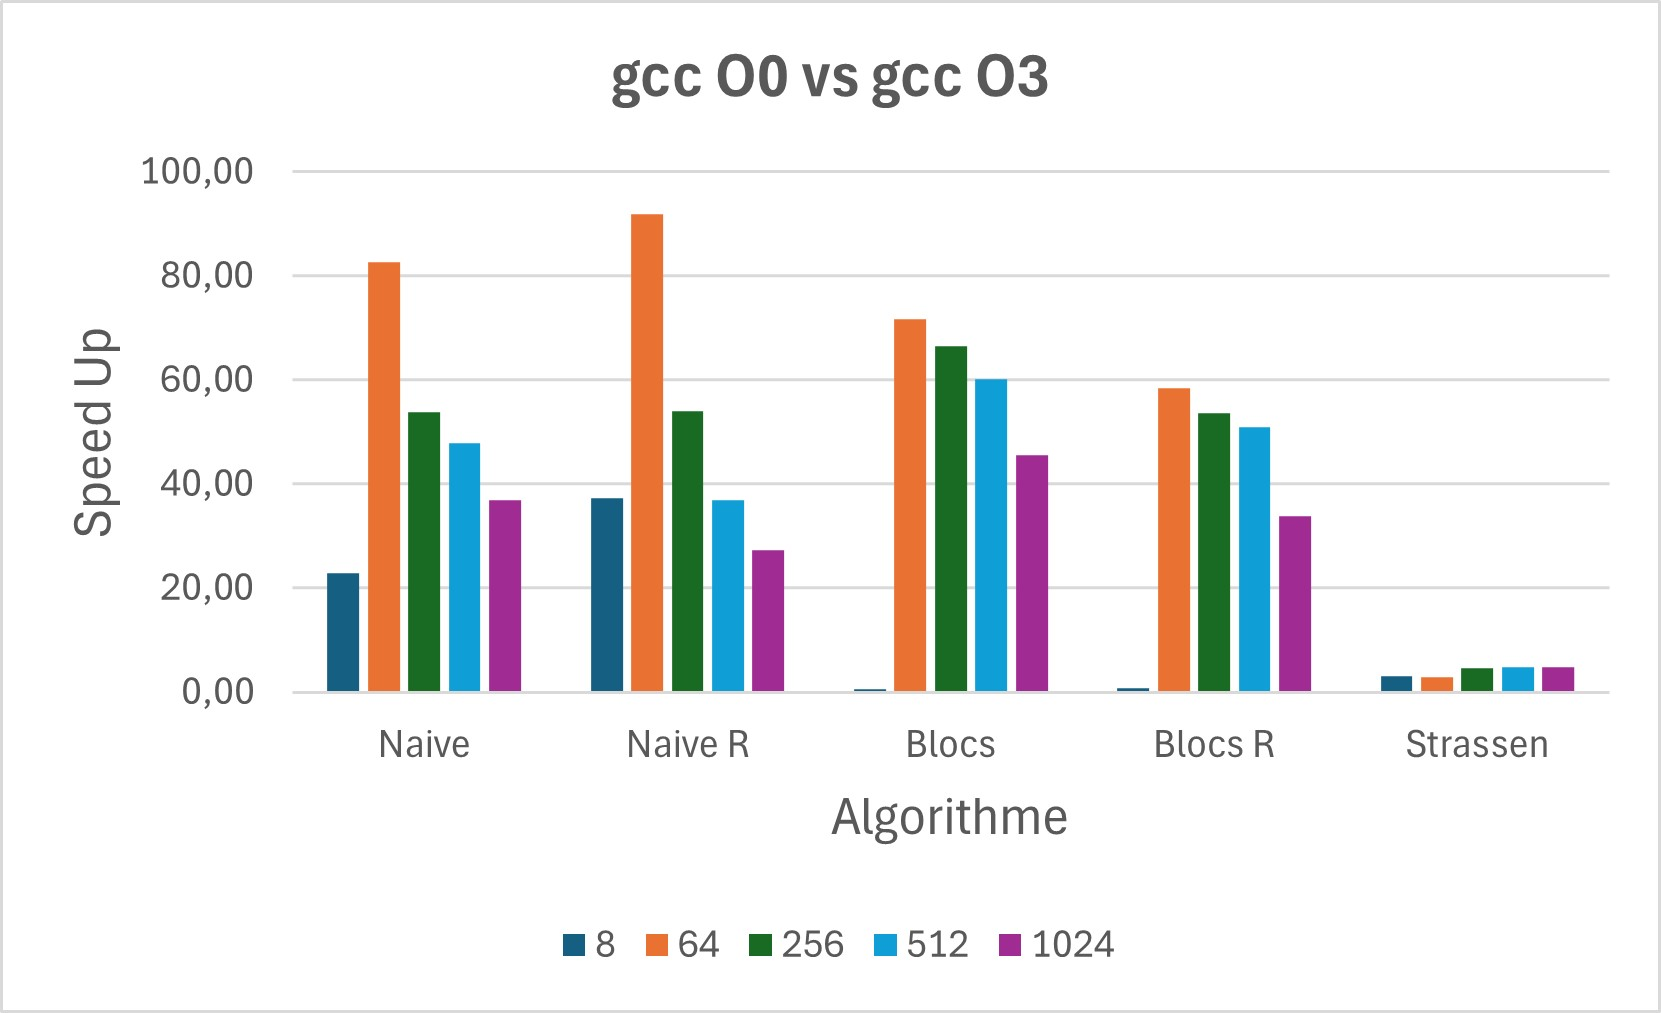
\includegraphics[width=1\columnwidth]{Images/SpeedUp1_gcc0vsgcc3.jpg}
    \caption{Speed Up de l'optimisation de gcc O3 par rapport à gcc O0.}
    \label{fig:4}
\end{figure}

Dans O3, qui applique les optimisations les plus agressives, telles que le déroulement des boucles et les optimisations au niveau de la vectorisation, les algorithmes de taille moyenne-grande (64x64 et 256x256) montrent une amélioration considérable, notamment dans les algorithmes tels que Naïve Reordered et par blocs réarrangés. Cependant, pour les petites matrices (8x8), les résultats sont plus petits, voire négatifs dans certains cas, probablement parce que la surcharge des optimisations dépasse les avantages pour les petits problèmes. Strassen n'en profite toujours pas autant, en raison de son approche récursive qui n'est pas idéale pour les optimisations agressives au niveau des boucles..

\subsection{Parallélisation par threads}

Ensuite, en utilisant l'optimisation gcc O3, nous avons commencé à utiliser des algorithmes de parallélisation, pour voir comment cela affecterait le comportement de nos algorithmes. Pour la parallélisation, \textbf{pragma} a été utilisé, ce qui permet d'exécuter certaines parties du code en parallèle, permettant ainsi de diviser le travail en plusieurs threads. Pour cette étude, seuls les algorithmes naïve, naïve réordonnés, blocs et blocs réordonnés ont été utilisés, puisque ce sont eux qui permettaient la parallélisation.

Dans la multiplication naïve, les deux premières boucles ont été parallélisées, qui parcourent respectivement les lignes et les colonnes de la matrice résultante. Les deux boucles ont été fusionnées en une seule boucle et réparties entre différents threads, permettant à chaque thread de calculer simultanément différentes parties du tableau.

Pour la multiplication des blocs, les boucles externes, qui parcourent les blocs de la matrice, ont été parallélisées, permettant à chaque thread d'être responsable du calcul d'un sous-ensemble de blocs en parallèle.

Le temps d'exécution du système avec l'optimisation O3 est indiqué ci-dessous, mais sans parallélisation, afin qu'il puisse être utilisé comme comparaison avec les résultats obtenus avec chacune des parallélisations.


\begin{figure}[H]
    \centering
    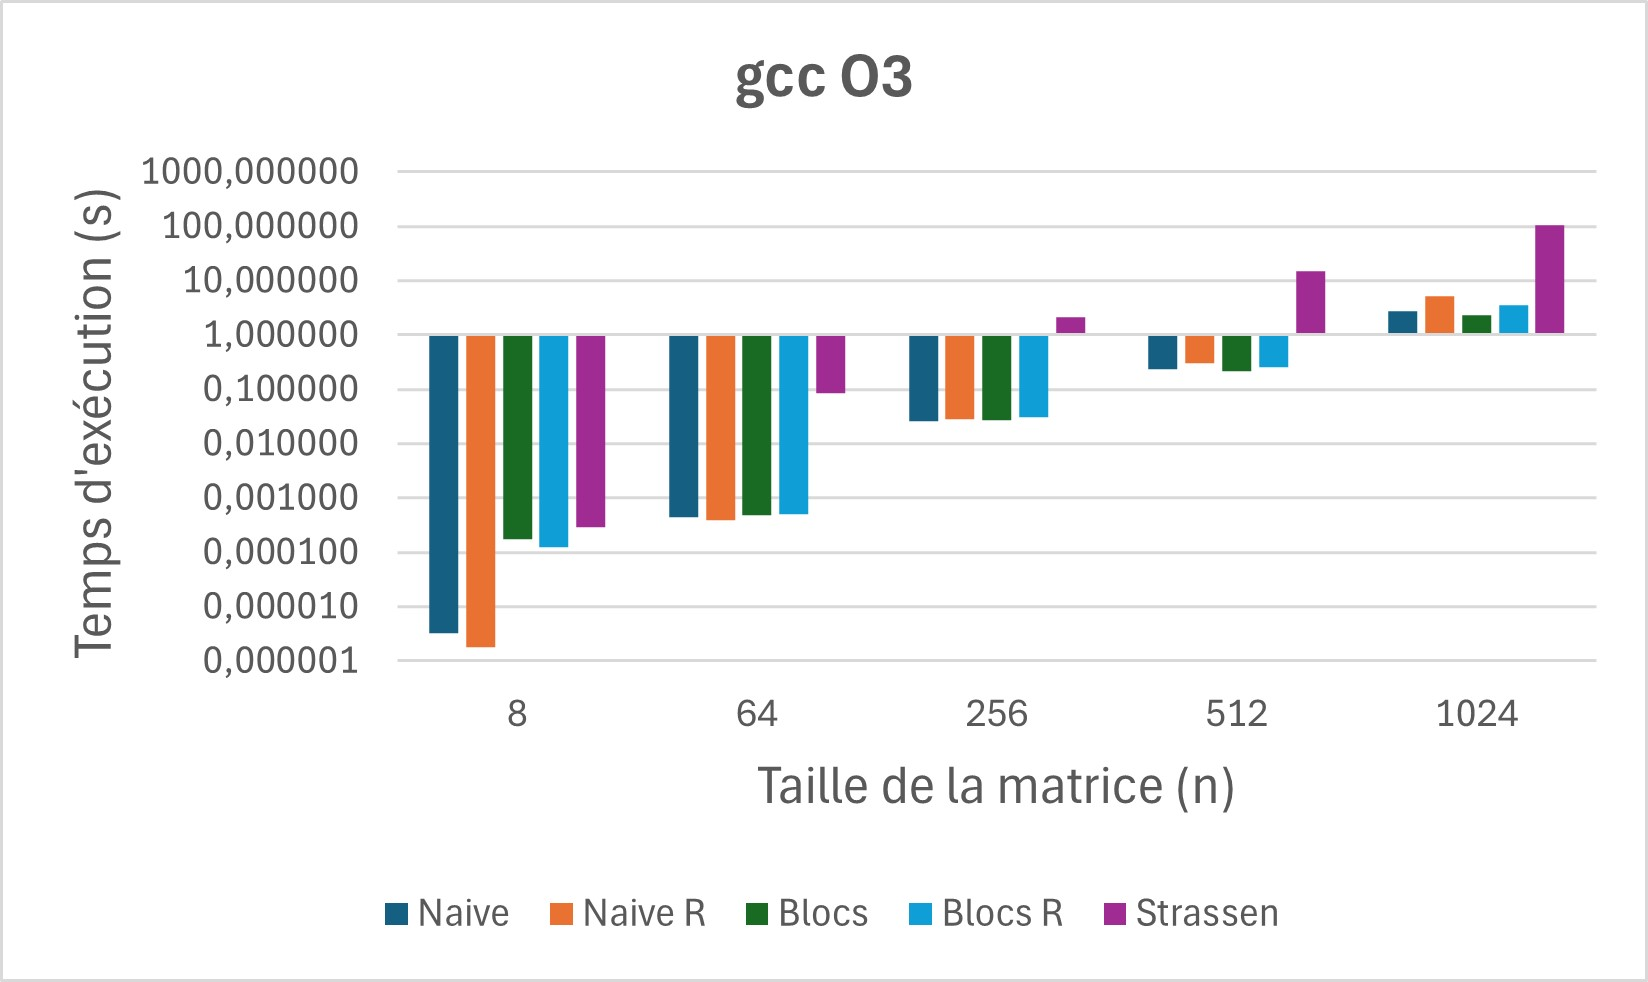
\includegraphics[width=1\columnwidth]{Images/Temps_gcc3.jpg}
    \caption{Temps d'exécution de l'algorithme avec optimisation gcc O3.}
    \label{fig:5}
\end{figure}


Les figures suivantes montrent les résultats de Speed Up pour les parallélisations de 2, 4 et 8 threads.


\subsubsection{Parallélisation avec 2 threads}

Ci-dessous les résultats.

\begin{figure}[H]
    \centering
    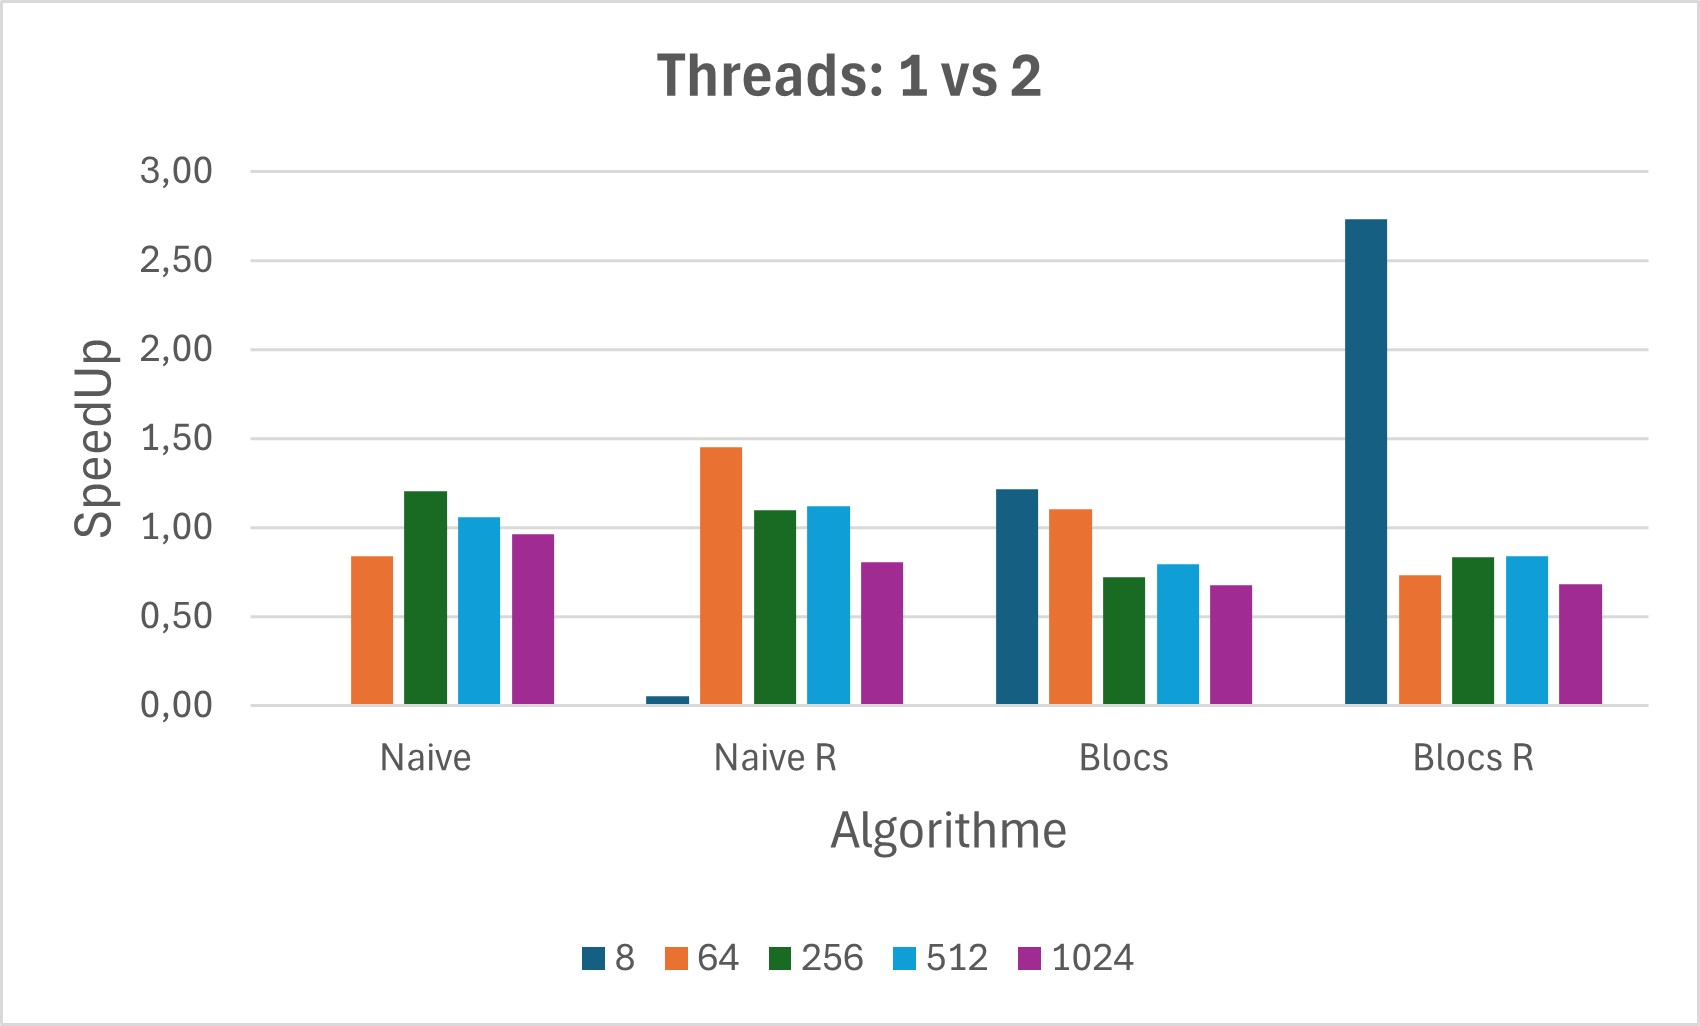
\includegraphics[width=1\columnwidth]{Images/SpeedUp1_Threads1vs2.jpg}
    \caption{Speed Up de la parallélisation à 2 fils par rapport au système non parallèle.}
    \label{fig:6}
\end{figure}


Avec seulement 2 threads, les résultats montrent que le parallélisme est plus efficace pour les algorithmes qui gèrent des blocs de données (notamment les « Blocs Réordonnés ») dans de petits tableaux. Ceci suggère que, pour les petites tailles, la localisation mémoire et la réduction des accès clairsemés permettent une meilleure utilisation de la parallélisation. Cependant, à des tailles plus grandes, l'avantage du parallélisme diminue, ce qui indique que la surcharge de synchronisation entre les threads et l'accès inefficace à la mémoire (en raison de petits caches ou d'un manque de prélecture appropriée) peuvent compenser les gains potentiels. Les algorithmes « naïfs » souffrent particulièrement de leur structure de boucle moins optimisée en termes de localisation des données.


\subsubsection{Parallélisation avec 4 threads}

Ci-dessous les résultats.

\begin{figure}[H]
    \centering
    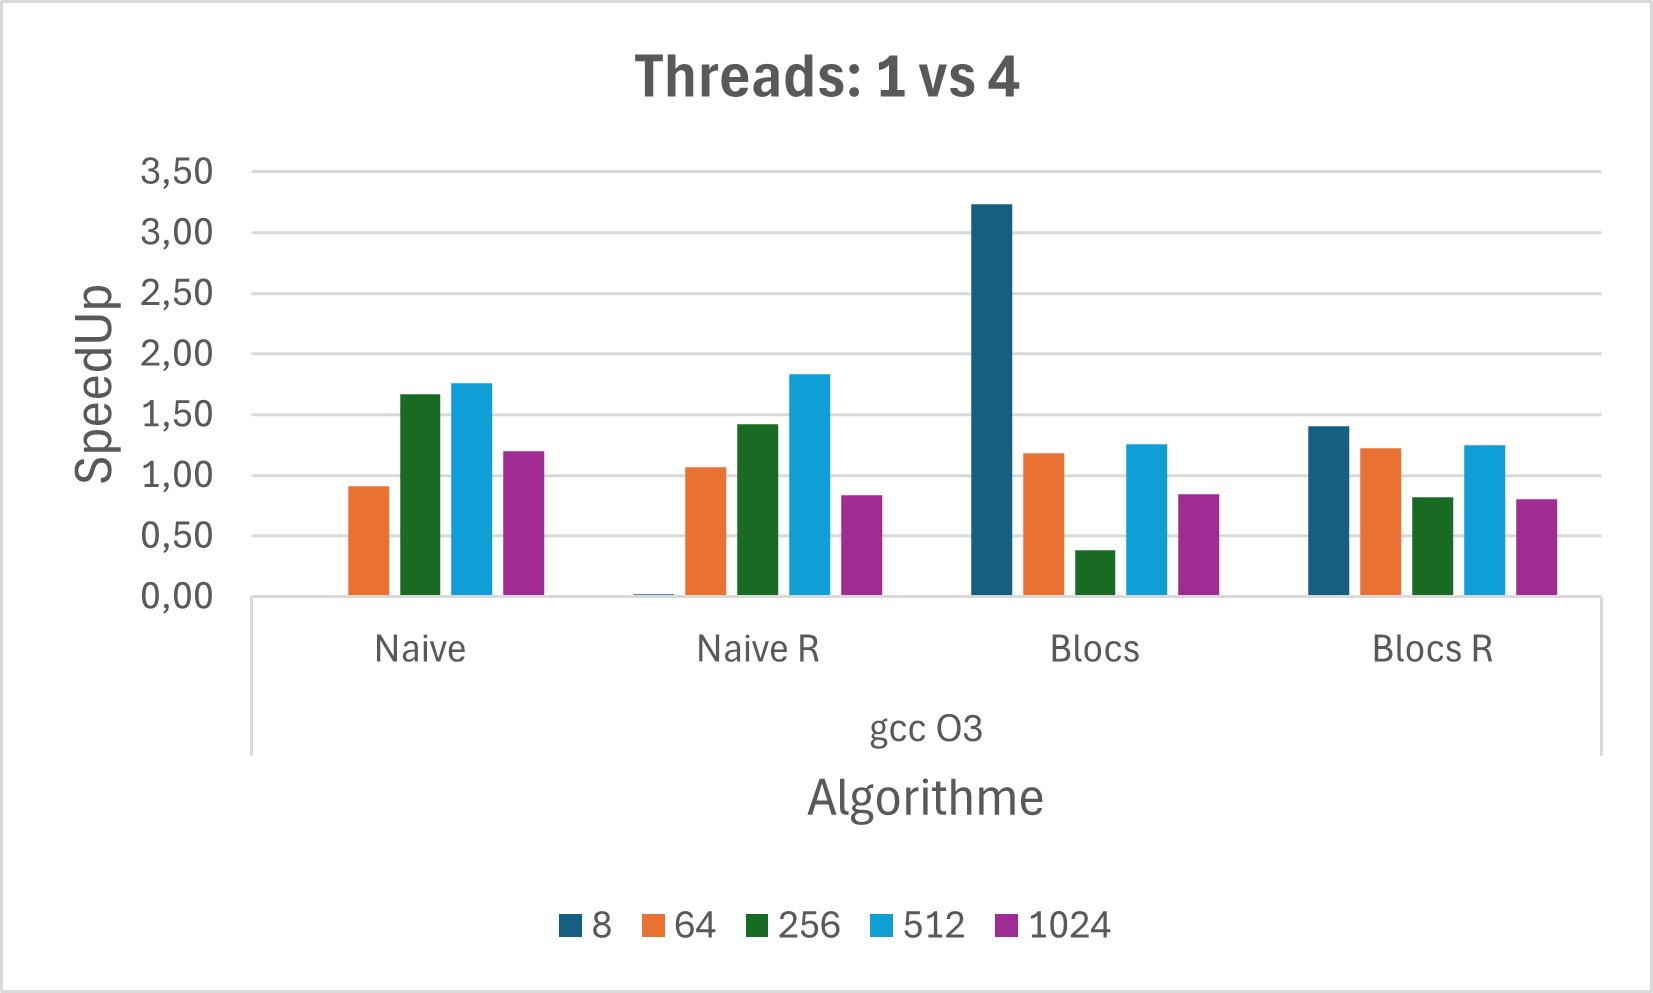
\includegraphics[width=1\columnwidth]{Images/SpeedUp1_Threads1vs4.jpg}
    \caption{Speed Up de la parallélisation à 4 fils par rapport au système non parallèle.}
    \label{fig:7}
\end{figure}

Avec 4 threads, les performances s'améliorent de manière plus significative dans les algorithmes de blocs sur des tableaux de petite et moyenne taille, ce qui indique que l'augmentation du nombre de threads permet d'exploiter davantage le parallélisme, même s'il existe toujours une limitation due à la gestion du cache et aux accès dans le désordre. mémoire. Pour les tailles moyennes (64x64 et 256x256), les algorithmes de blocs ne s'améliorent pas proportionnellement, ce qui suggère que les threads pourraient être en compétition pour les ressources mémoire ou que la division du tableau n'est pas suffisamment granulaire pour éviter des conflits dans l'utilisation du cache. L'effondrement des performances des algorithmes de Naïve Reorder à grande taille indique que, même si des threads supplémentaires sont disponibles, le manque de cohérence dans les accès mémoire et la structure des boucles reste un goulot d'étranglement.

\subsubsection{Parallélisation avec 8 threads}

Ci-dessous les résultats.

\begin{figure}[H]
    \centering
    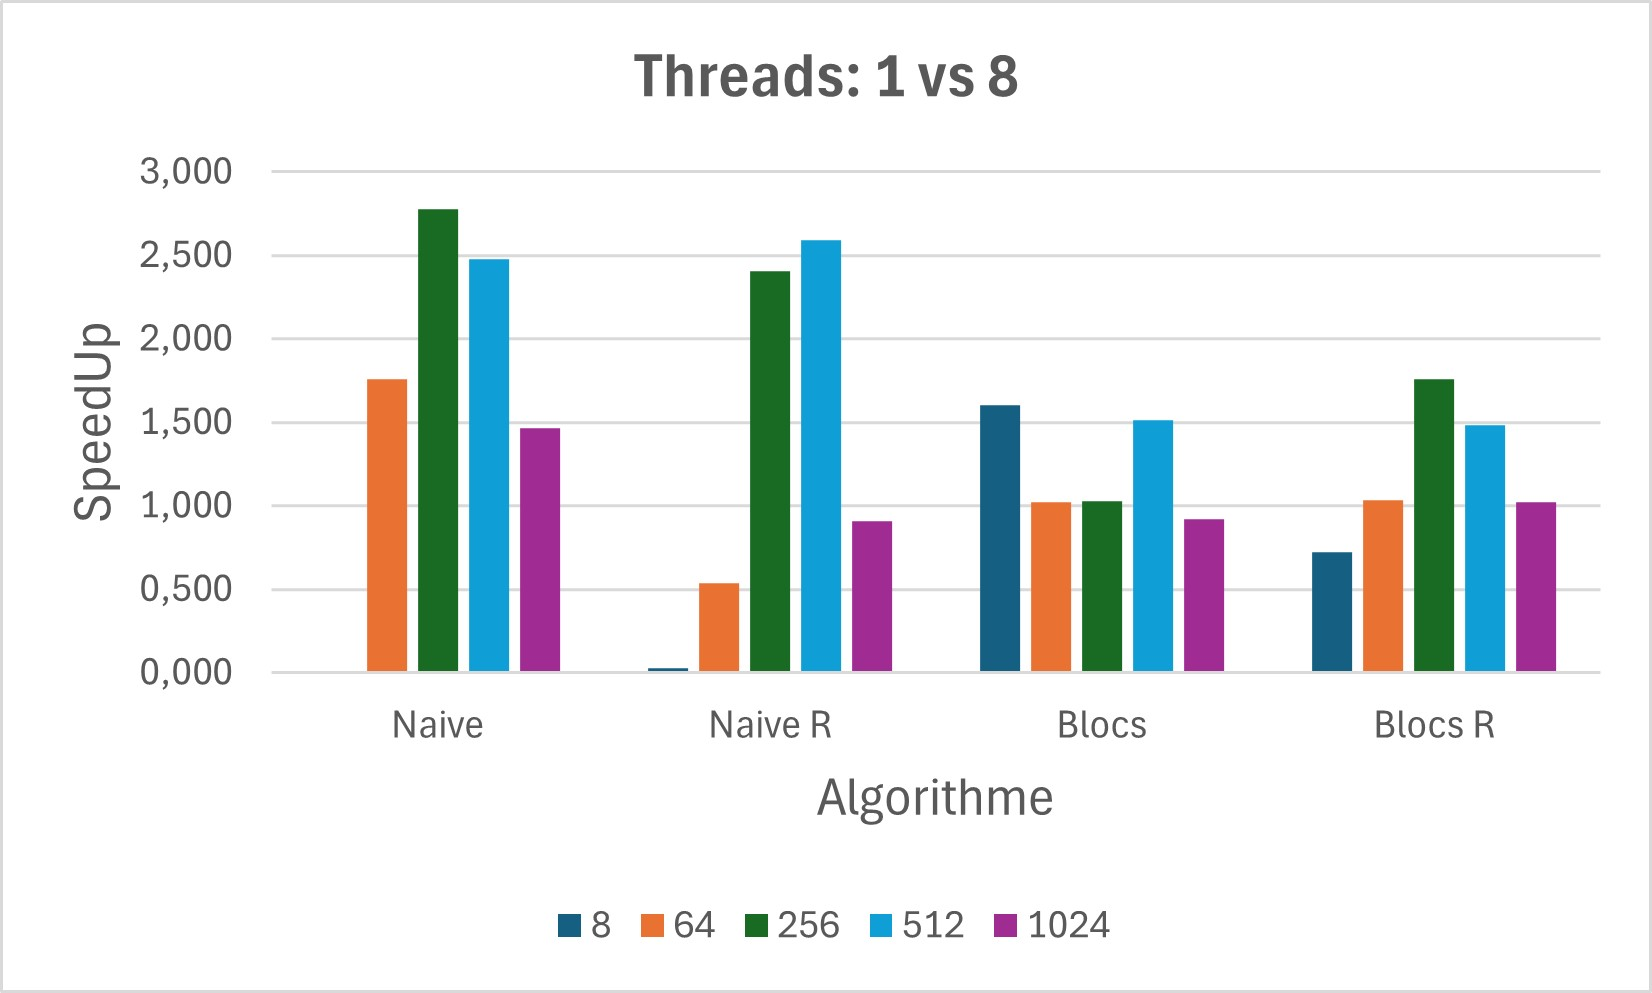
\includegraphics[width=1\columnwidth]{Images/SpeedUp1_Threads1vs8.jpg}
    \caption{Speed Up de la parallélisation à 8 fils par rapport au système non parallèle.}
    \label{fig:8}
\end{figure}

Avec 8 threads, le parallélisme atteint son potentiel maximum dans les tailles moyennes (256x256 et 512x512), où des algorithmes comme Naïve Reordered et Blocks Reordered obtiennent une bonne accélération, ce qui suggère que les sous-matrices sont suffisamment grandes pour permettre aux threads de fonctionner en parallèle. efficacement sans interférence significative dans le cache ou la mémoire. Cependant, les performances sur les petites baies (8x8) sont très faibles, ce qui signifie que la surcharge liée à la gestion de 8 threads est trop élevée pour la petite quantité de travail pouvant être parallélisée à cette taille. Pour les très grands tableaux (1 024 x 1 024), l'augmentation des threads ne produit pas une accélération substantielle, ce qui peut indiquer que l'architecture de la mémoire n'évolue pas bien avec autant de threads ou que l'efficacité de la parallélisation est réduite par le volume de transferts de données par rapport à la mémoire. coût de calcul.

\subsection{SIMD}

SIMD (Single Instruction, Multiple Data) est un type de parallélisme au niveau des données dans lequel une seule instruction est appliquée simultanément à plusieurs données à la fois. Il est utilisé pour accélérer le traitement des tâches impliquant de grands ensembles de données.

Les résultats de Speed Up utilisant SIMD et l'optimisation O3 des algorithmes naïve, naïve réorganisés, blocs et blocs réorganisés, comparés aux résultats obtenus uniquement avec l'optimisation gcc O3, peuvent être vus ci-dessous.


\begin{figure}[H]
    \centering
    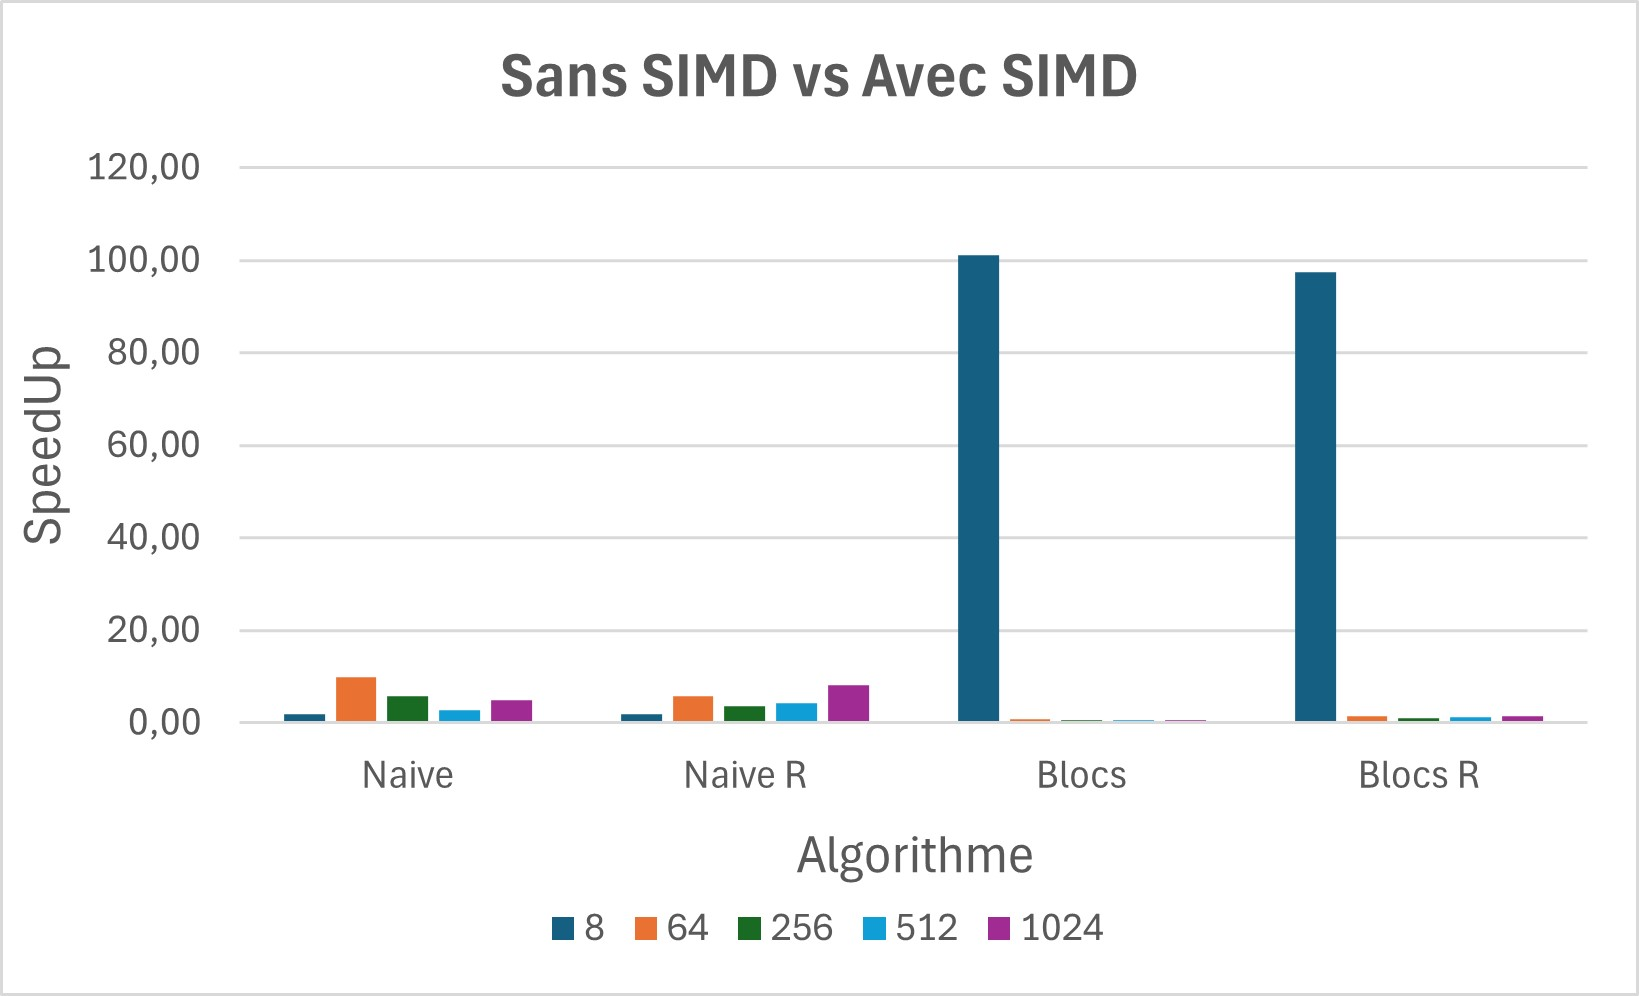
\includegraphics[width=1\columnwidth]{Images/SpeedUp1_SIMD.jpg}
    \caption{Speed Up en utilisant SIMD.}
    \label{fig:9}
\end{figure}

Sur de petites matrices (8x8), l'utilisation de SIMD génère une accélération massive des algorithmes de blocs, avec des améliorations allant jusqu'à 100x par rapport à son homologue non-SIMD. En effet, SIMD est extrêmement efficace lorsque les données sont bien alignées et que la taille du bloc est suffisamment petite pour que plusieurs éléments puissent être traités en parallèle en un seul cycle. Les algorithmes Naïve et Naïve Reordering en bénéficient également, mais dans une moindre mesure, ce qui indique que l'accès non séquentiel et la structure en boucle limitent la capacité du SIMD à exploiter le parallélisme.

Pour les matrices moyennes (64x64), les algorithmes Naïve montrent toujours une amélioration significative par rapport à SIMD, tandis que les algorithmes blocs constatent même une dégradation. Cela suggère que les modèles d'accès dans les algorithmes de blocs ne sont pas bien adaptés aux opérations vectorisées, probablement en raison d'un mauvais alignement des données ou d'une fragmentation excessive qui empêche SIMD de fonctionner de manière optimale. À ces tailles, la charge de réorganisation des données pour SIMD peut dépasser les avantages du parallélisme.

Sur les grandes matrices (256x256 et plus), les algorithmes de blocs affichent une accélération marginale, voire des pertes de performances, lors de l'utilisation de SIMD. Cela peut être lié à la pression exercée sur le cache et au manque de localité des données, ce qui réduit l'efficacité du parallélisme au niveau des données fourni par SIMD. En revanche, les algorithmes Naïve et Naïve Reordered affichent une augmentation de performances plus soutenue, ce qui indique qu'à ces tailles, la parallélisation au niveau des instructions est mieux appliquée en raison de la simplicité de ses opérations par rapport aux algorithmes par blocs, qui souffrent du désordre dans l'accès à la mémoire.


\subsection{Profondeur de récursion de Strassen}

Enfin, pour l’algorithme de Strassen, il a été vérifié comment le changement de profondeur de récursion affectait le comportement de l’algorithme.
La profondeur de récursion dans l'algorithme de Strassen fait référence au nombre de fois que l'algorithme se décompose de manière récursive avant d'atteindre un cas de base dans lequel une multiplication matricielle plus simple est effectuée.

La profondeur de la récursion dépend du nombre de fois que vous pouvez continuer à diviser les tableaux avant d'atteindre le cas de base. Ce processus est répété jusqu'à ce que la taille des sous-matrices atteigne une petite valeur, généralement lorsque n=1, mais il peut être arrêté avant d'utiliser une multiplication naïve pour de petites tailles.

Ci-dessous, dans le tableau, vous pouvez comparer les temps d'exécution de différentes profondeurs de récursion pour différentes tailles de matrice.

\begin{figure}[H]
    \centering
    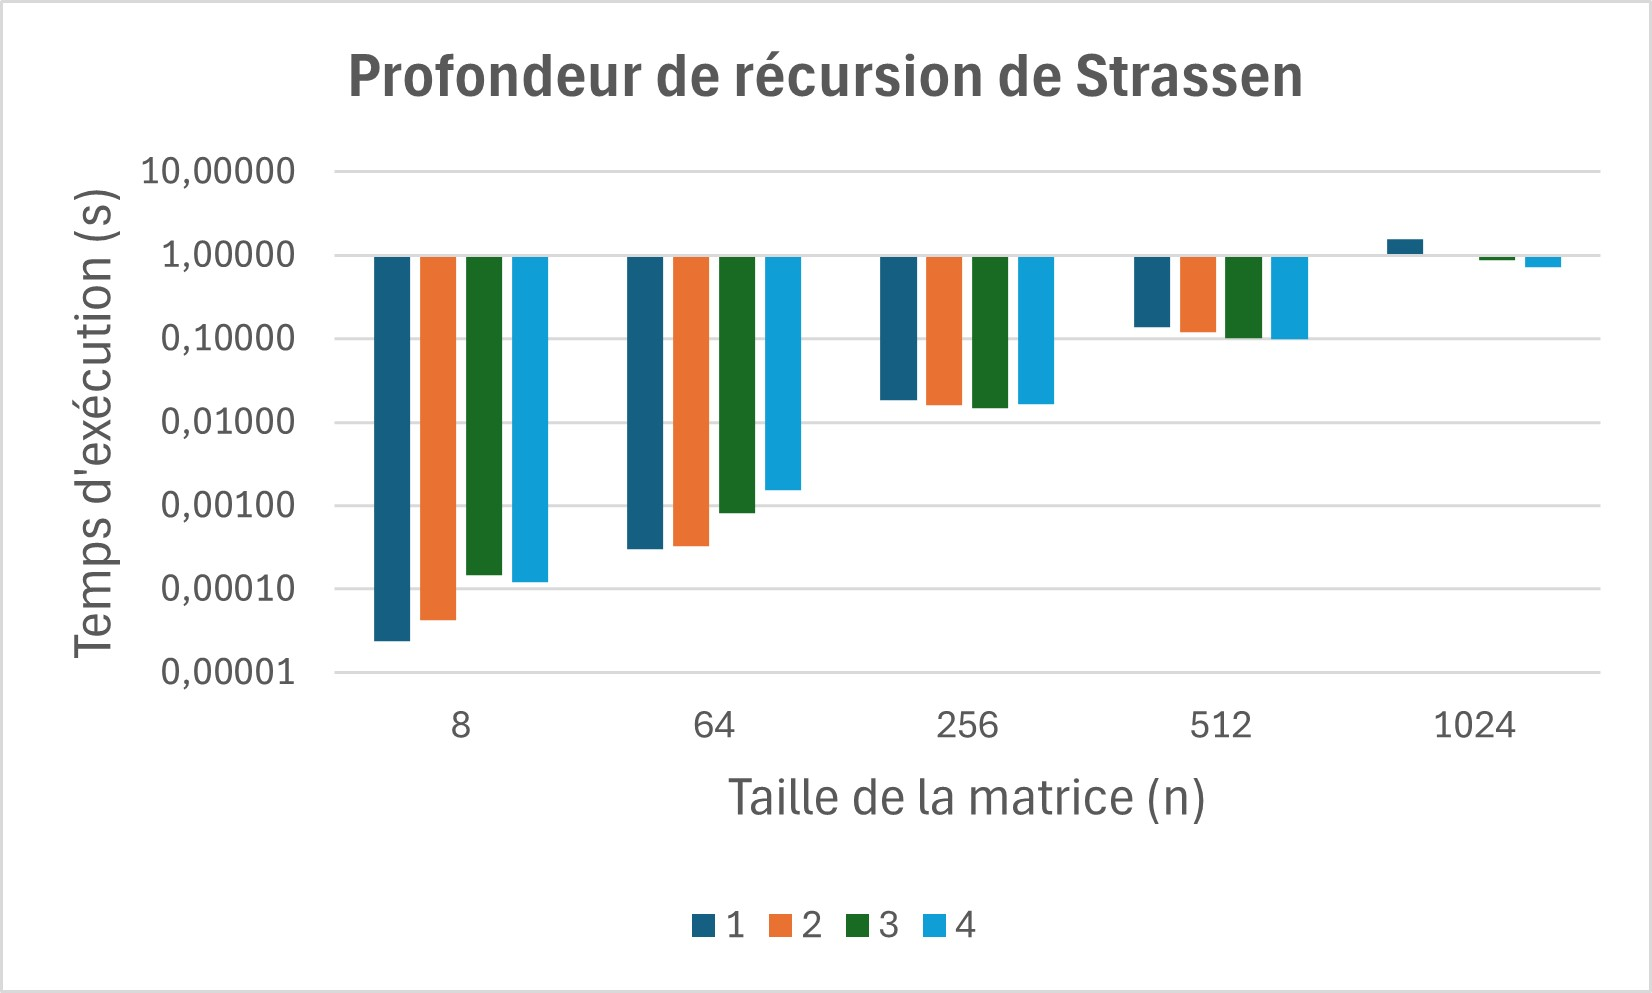
\includegraphics[width=1\columnwidth]{Images/Temps_Strassen_Recurtion.jpg}
    \caption{Temps d'exécution pour différentes profondeurs de récursion dans l'algorithme de Strassen.}
    \label{fig:10}
\end{figure}

Le temps d'exécution de Strassen s'améliore à mesure que la profondeur de récursion augmente, en particulier sur les grandes matrices (1024 et 512), où une plus grande profondeur réduit le temps. En effet, la décomposition des matrices en sous-problèmes plus petits permet de mieux utiliser les optimisations et l'efficacité du cache. Cependant, pour les petites matrices (8 et 64), une plus grande profondeur de récursion n'est pas aussi bénéfique et peut même aggraver légèrement le temps, puisque la surcharge de division des matrices dépasse les gains de parallélisme dans ces cas.

\end{document}
